\chapter{Removing detuning distortions of wrapped phase by using robust 
 quadrature filters}

%\section{abstract}One of the most common and least desirable problems with
%the 
%demodulated phase in interferometry is the detuning error. Detuning error is 
%the distortion that we obtain when the demodulation algorithm is not well 
%calibrated, or when the object under test is not completely static. In this 
%paper, we propose an interesting method to remove the detuning distortions
%from 
%the wrapped phase obtained by the uncalibrated phase interferometry 
%demodulation methods. The method presented here takes the local frequencies as 
%a priori knowledge from the wrapped phase, and uses an iterative approach to 
%refine the phase. Here, we show that with this practical strategy we are able 
%to remove detuning distortions from the demodulated wrapped phase. Tests and
%results from simulated and experimental data will be shown.
One of the most common and least desirable problems with the 
demodulated phase in interferometry is the detuning error. Detuning error is 
the distortion that we obtain when the demodulation algorithm is not well 
calibrated, or when the object under test is not completely static. In this 
chapter, we propose an interesting method to remove the detuning distortions from 
the wrapped phase obtained by the uncalibrated phase interferometry 
demodulation methods. The method presented here takes the local frequencies as 
a priori knowledge from the wrapped phase, and uses an iterative approach to 
refine the phase. Here, we show that with this practical strategy we are able 
to remove detuning distortions from the demodulated wrapped phase. Tests and
results from simulated and experimental data will be shown.

%\ocis{120.3180, 120.3940, 120.2650, 120.5050.}
%%  The method presented here uses an iterative robust quadrature filter that
%%  takes the gradient of the previous demodulated phase as \emph{a priori} 
%%  knowledge of the local frequencies. This method is stable and converges in
%%  few iterations. This way, we are able to filter out the detuning distortions
 
%%  present in the demodulated phase. To show its performance, we are going
%%  to show tests and results from experimentally obtained insterferograms. 



\section{Introduction}
In optical interferometry tests, the modulating phase has the information of
interest. Therefore, estimating the phase with the least possible error is the 
most important task in interferometry. However, this is not always possible, 
and one of the most common errors of phase interferometry demodulation 
algorithms (PIDA) is the so-called detuning error 
\cite{Malacara,GeneralTheory,Mosino:09, fringePatternAnalisys}. In literature,
we can find several works that study and measure the effects of the detuning
error and the factors that cause it \cite{PhaseDetuning_0, PhaseDetuning_1, 
Malacara, Mosino:10, ShopTesting, AccuracyPSI_1, deGroot:95,
Schmit:95, Gutmann:98, Servin:10}. For example, in phase shifting
interferometry, if the object under test is not static or the piezoelectric
transducer used to introduce the phase shifts is incorrectly calibrated, the
PIDA produces a detuning error. 
%%To avoid this detuning errors in PSI, digitally speaking, iterative 
%%algorithms 
%%have been proposed to tune in the phase shifting algorithm with the 
%%interferogram sequence in order to recover a more accurate modulating phase 
%%\cite{Morgan,Okada,Kong,Wang_AIA,Mariano,self_tuning,Medina,RAPS}.
Another example where this detuning error commonly occurs is in dynamic 
interferometry. In dynamic interferometry, detuning error occurs when we 
do not have fast enough cameras or high repetition lasers with long coherence 
lengths, or a combination of both. In the Fourier method, the detuning error is 
present when the filtering process can not be performed properly, since the 
carrier is not enough to separate the complex signal in the Fourier domain. 
Therefore, in general, when the PIDA does not receive the interferogram or 
interferograms as expected, it recovers a modulating phase with detuning error.

This detuning error is present in the demodulated phase as a low powered 
signal having twice the frequency than the interferograms under analysis.
Mosi\~no et al. \cite{Mosino:09} demonstrate that this detuning error can be 
described by the following expression: 
\begin{equation}\label{Eq:DetuningError}
	\Delta \phi \approx - \frac{\varepsilon}{c} \sin(2\phi),
\end{equation}
where $\Delta \phi$ is the difference between the desired phase $\phi$ and the 
erroneous spurious phase $\phi^\varepsilon$, $\varepsilon$ is the erroneous 
spurious signal that our PIDA does not remove properly, and $c$ is the complex 
desired signal we want to recover. This detuning effect is graphically shown in 
the unwrapped phase of Fig. \ref{fig:SimulatedPhase3D}(a). As we see, the 
distorted phase has a double frequency component mounted, while the desired 
unwrapped phase has to look like the one in Fig. \ref{fig:SimulatedPhase3D}(b). 
%Thus, removing the detuning error without affecting the 
%information of interest is almost impossible by filtering the wrapped 
%phase with common low-pass filters, since the spurious signal and the $2\pi$ 
%phase jumps.
%Another more clever approach is filtering the wrapped phase as follows:
%\begin{equation}
%	\hat{\phi} = \arctan \left[ \frac{\sin(\phi^\varepsilon) * h}
%	{\cos(\phi^\varepsilon) * h} \right],
%\end{equation}
%where $*$ is the convolution operator, $h$ is a low-pass convolution 
%kernel, $\phi^\varepsilon$ is the wrapped phase with detuning distortions 
%and $\hat \phi$ is the filtered wrapped phase. The problem with this 
%approach is that the filter removes phase information before lessen the 
%detuning error.
Therefore, removing the detuning error from the wrapped phase without affecting 
the information is not a trivial problem, and, as far as we know, there is no 
published work on processing the distorted wrapped phase in order to reduce 
this detuning error.

Hence, in this chapter, we are going to show how we can reduce this detuning 
error from the demodulated wrapped phase by using a variant of the RQF 
\cite{RQF}. The variant that we implement here is 
such that the RQF use the gradient of the distorted demodulated wrapped 
phase as \emph{a priori} local frequency information. As we work with a 
wrapped phase, the data term of the RQF compares the complex signal of 
this wrapped phase with the signal that we are expecting to obtain; that is, 
the one without distortions.
%%Additionally, 
%%we generate a complex signal with the demodulated wrapped phase and 
%%process it with this variant of the RQF to obtain a more refined 
%%demodulated phase.
To show the performance of the phase detuning correction method (PDCM)
presented here, we will present test and results from simulated and 
experimentally obtained data.

\begin{figure*}[th!]
  \begin{center}
    \begin{tabular}{ c c }
      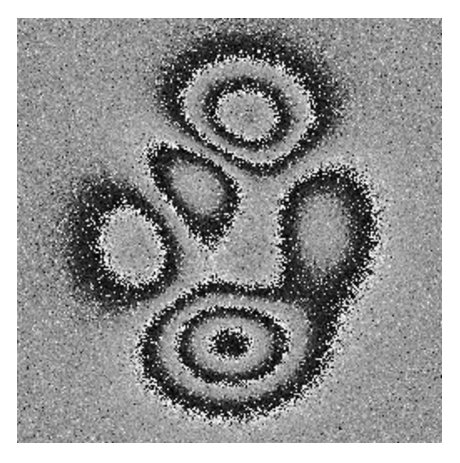
\includegraphics[scale=0.75]{Chpt4_figures/Fig_1aNoise.eps}&
      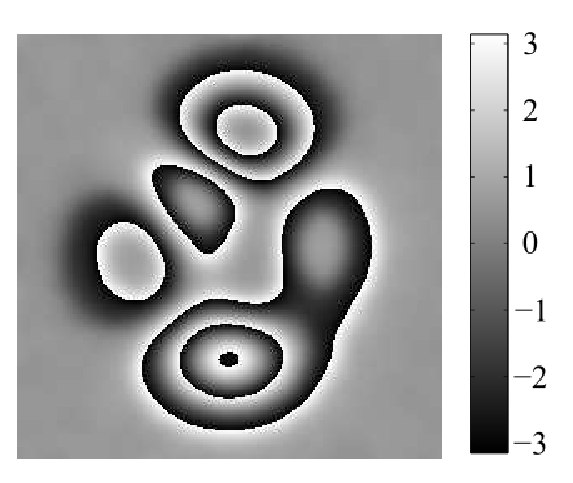
\includegraphics[scale=0.75]{Chpt4_figures/Fig_1bNoise.eps}\\
      (a) &  (b)
    \end{tabular}
  \end{center}
  \caption{Simulated wrapped phase comparison. (a) Synthetic input wrapped 
  phase with detuning error. (b) Recovered wrapped phase map using the proposed 
  PDCM.}
  \label{fig:SimulatedPhaseComparison}
\end{figure*}

\begin{figure*}[th!]
  \begin{center}
      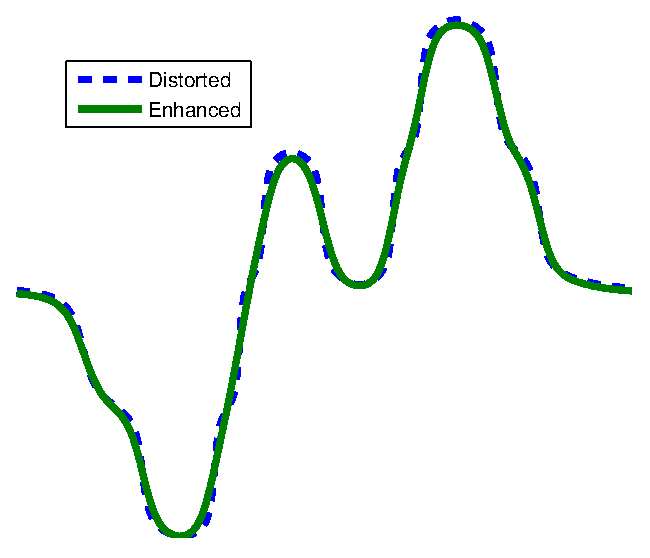
\includegraphics[scale=0.75]{Chpt4_figures/2D_error.eps}
  \end{center}
  \caption{Comparison between an unwrapped row of the distorted input 
  and the enhanced phase; the dashed line is the unwrapped phase with detuning 
  error, and the solid line is the unwrapped phase processed with the PDCM. 
  Note: The noise had been removed from the original distorted wrapped
  phase in Fig. \ref{fig:SimulatedPhaseComparison}(a) for clarity and
  comparison purposes.}
  \label{fig:SimulatedPhaseComparisontemp}
\end{figure*}

\section{Phase Detuning Correcting Method (PDCM)}
As we said above, our PDCM uses a specially tuned RQF system to process a 
complex signal generated by the given demodulated wrapped phase. The energy
function of this specially tuned RQF is the following:
\begin{eqnarray}\label{Eq:U(f)}
U(f) &=& \sum_{x,y\in L} \mid f(x,y) - 2 g(x,y) \mid ^2 +\lambda \sum_{x,y\in L} 
  \mid f(x,y) - f(x-1,y) e^{i u_{x,y}} \mid^2 \nonumber\\
  & & + \lambda \sum_{x,y\in L} \mid f(x,y) - f(x,y-1) e^{i v_{x,y}} \mid^2,
\end{eqnarray}
where $g(x,y)= e^{i \phi^\varepsilon_{x,y}}$ is the complex
signal generated by the demodulated wrapped phase $\phi^\varepsilon_{x,y}$
that we are going to process, $f(x,y)$ is the independent complex value 
that minimizes Eq. (\ref{Eq:U(f)}) (and hence, the output of our PDCM), 
$\lambda$ is the regularization parameter that controls the bandwidth of the 
quadrature filter, and $u_{x,y}$ and $v_{x,y}$ are the a priori local frequency 
information obtained from the wrapped phase; 
%%are the differences of $\phi^\varepsilon_{x,y}$ 
%%with respect to $x$ and $y$ respectively.
that is, $u_{x,y}$ and $v_{x,y}$ are the $x$ and $y$ components of the 
gradient of $\phi^\varepsilon_{x,y}$. 
Below, we will show how this prior information is obtained from the wrapped
phase $\phi^\varepsilon_{x,y}$. The sums run over all valid sites $x,y$ in 
$L$, being $L$ the lattice domain of the demodulated wrapped phase. To minimize 
Eq. (\ref{Eq:U(f)}), one could use any method for solving systems of 
linear equations; in particular, we use the \emph{Gauss-Seidel} method. 
Having the complex field $\hat f$ that minimizes Eq. (\ref{Eq:U(f)}), the 
refined demodulated wrapped phase is obtained as before

\begin{equation}
	\hat{\phi}_{x,y}=arg[\hat{f}(x,y)];\label{Eq:phi}
\end{equation}
that is, as the angle of the complex signal $\hat f$ obtained by the
minimization process.

The new wrapped phase $\hat \phi$, estimated with Eq. (\ref{Eq:phi}), is an 
improved version of our input wrapped phase $\phi^\varepsilon$; i.e., the 
detuning error has been lessened. If we use this process recursively, we can 
refine the wrapped phase until we obtain an almost error free enhanced wrapped 
phase. Using this approach, we ensure that the new calculated phase is almost 
free of detuning errors. Then, this recursive process can be given as: 
\begin{itemize}
\item[1.-] Estimate local frequencies $u$ and $v$ taking the wrapped
  gradient of the input wrapped phase $\phi^\varepsilon$
  [Eqs. (\ref{Eq:explicit_u}) and (\ref{Eq:explicit_v})].
\item[2.-] Take $\hat{f}$ that minimizes Eq. (\ref{Eq:U(f)}) using $u$, 
 $v$ and $g=e^{i \phi^\varepsilon}$ as data input.
\item[3.-] Calculate an enhanced $\phi$ using $\hat{f}$ with
  Eq. (\ref{Eq:phi}).
\item[4.-] Recalculate local frequencies $u$ and $v$ with the new
  wrapped phase $\phi$.
\item[5.-] Repeat steps $2$ to $4$ until a desired convergence point.
\end{itemize}

This convergence point can be given as the relative error between the 
former and the new wrapped phases in the following way:
\begin{equation}
	\varepsilon = \sum_{x,y} \left| \phi_{x,y}^{+} - \phi_{x,y}^{-} 
	\right|,
\end{equation}
where $\phi_{x,y}^{+}$ and $\phi_{x,y}^{-}$ are the wrapped phases obtained in 
the current and previous iterations, respectively. At the end of this 
iterative process, the new wrapped phase $\phi$ will be a wrapped phase without 
detuning distortions and without noise.

\begin{figure}[Ht]
  \begin{center}
    \begin{tabular}{ c c }
     
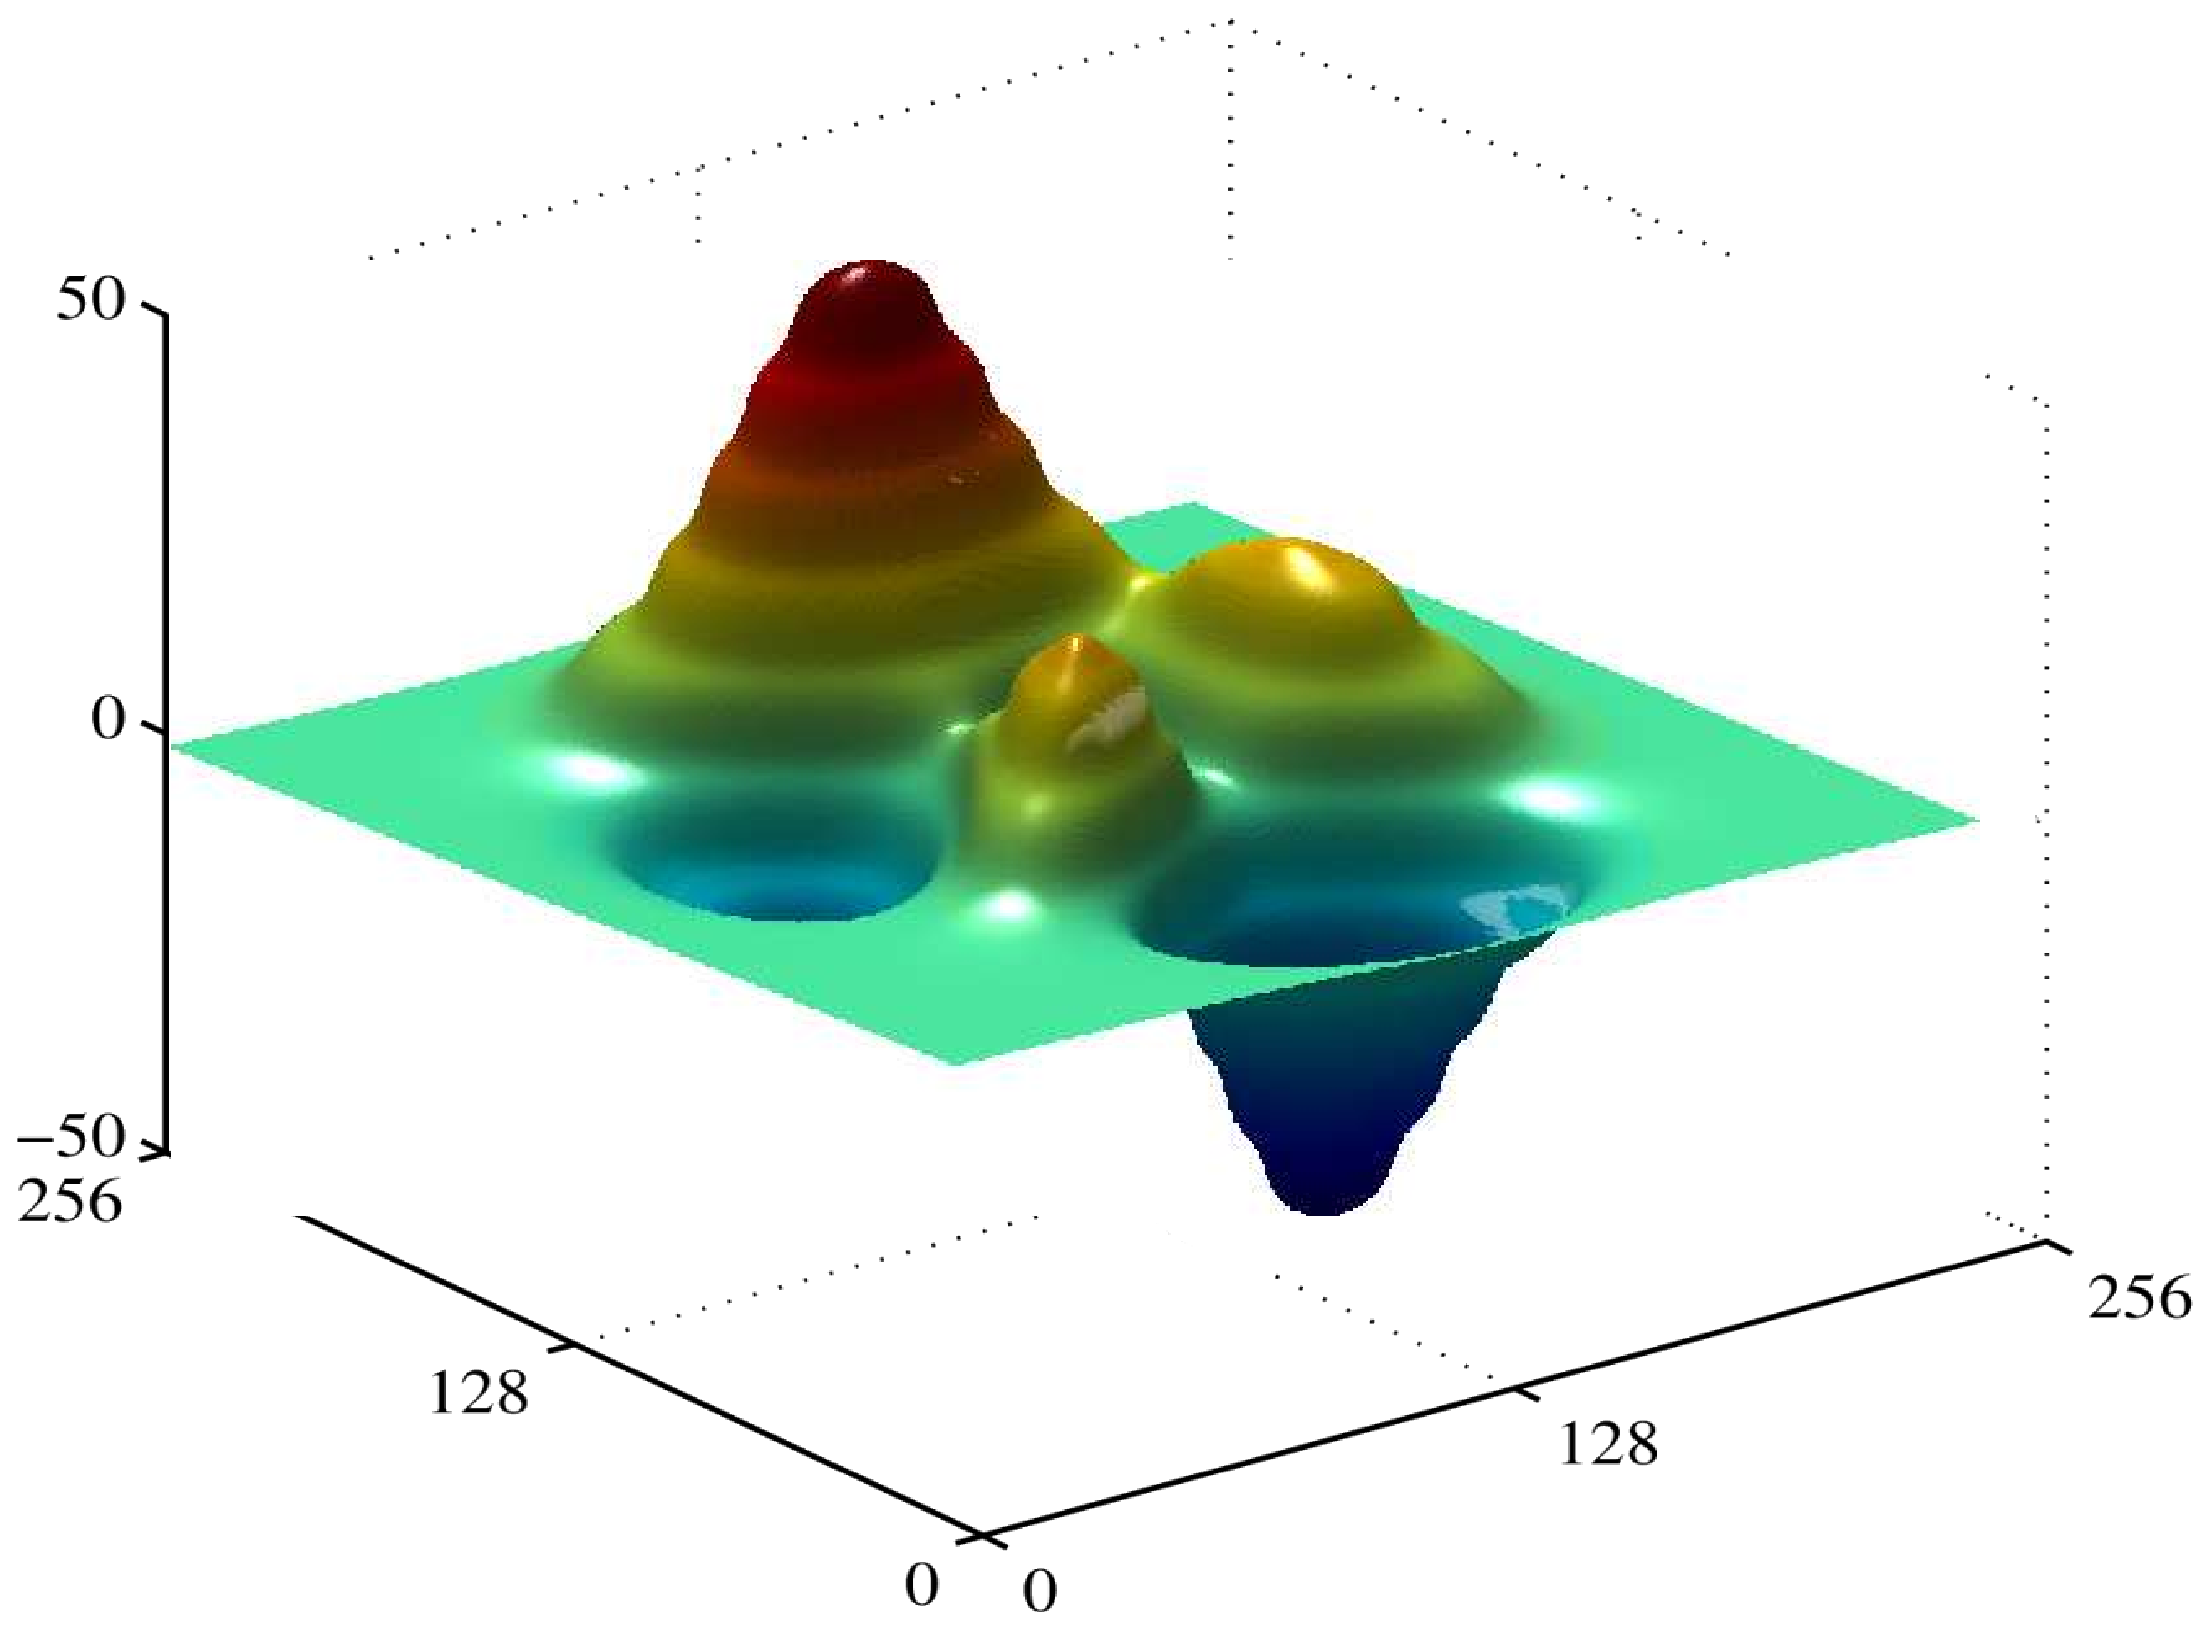
\includegraphics[width=.47\columnwidth]{Chpt4_figures/FaseError_Ideal_3D.eps}&
      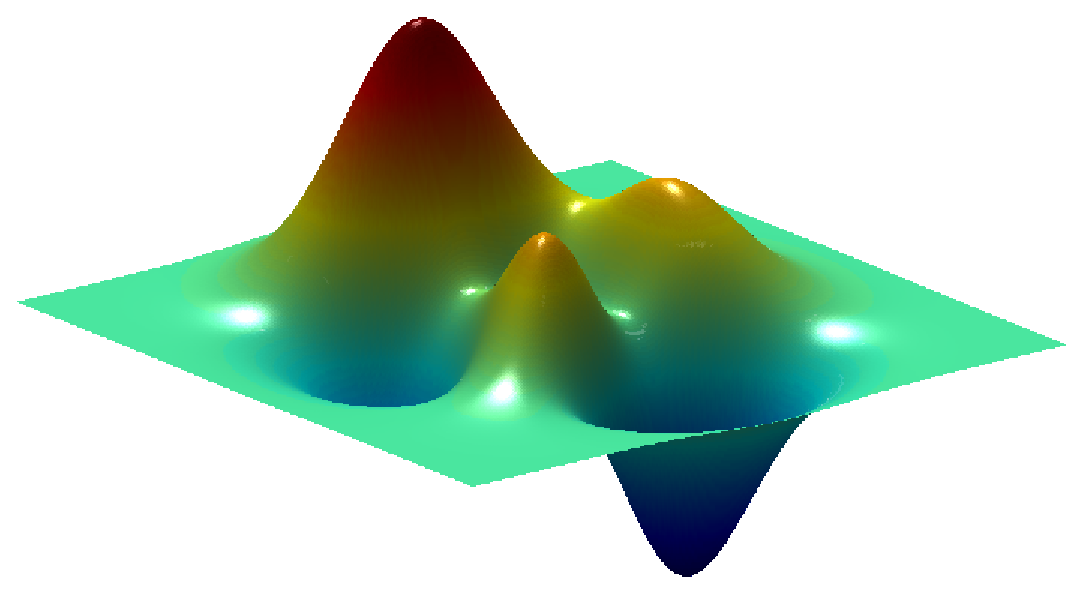
\includegraphics[width=.47\columnwidth]{Chpt4_figures/Fase_Ideal_3D.eps}\\
      (a) &  (b)\\
    \end{tabular}
  \end{center}
  \caption{Unwrapped simulated phase comparison of Fig. 
  \ref{fig:SimulatedPhaseComparison}. (a) Shows the 
  unwrapped phase with detuning error of Fig.
  \ref{fig:SimulatedPhaseComparison}(a). (b) Shows the recovered unwrapped 
  phase of Fig. \ref{fig:SimulatedPhaseComparison}(b) after using the proposed 
  PDCM. Note:  The noise had been removed from the original distorted wrapped
  phase in Fig. \ref{fig:SimulatedPhaseComparison}(a) for clarity and
  comparison purposes.}
  \label{fig:SimulatedPhase3D}
\end{figure}

\section{A priori local frequency calculation}

Since in order to calculate the local frequencies we have a wrapped phase, we
can not use finite differences directly due to the $2\pi$ phase jumps of the
wrapped phase. To estimate the local frequencies correctly, we propose taking
the gradient in an explicit way from the complex field as follows:
\begin{equation}\label{Eq:ExplicitGradient}
  \nabla \phi_{x,y} = \nabla \left[ \arctan \left(\frac{\sin{\phi_{x,y}}}	
      {\cos{\phi_{x,y}}}\right)\right].
\end{equation}
Therefore, differentiating Eq. (\ref{Eq:ExplicitGradient}) and 
simplifying, we obtain the following mathematical expression for local 
frequencies $u_{x,y}$ as
\begin{eqnarray}\label{Eq:explicit_u}
  u_{x,y} = \frac{\sin \phi \frac{\partial}{\partial x}  \cos \phi - \cos 
  \phi \frac{\partial}{\partial x} \sin \phi}{ \cos^2 \phi + \sin^2 \phi 
  },
\end{eqnarray}
and in a similar way, the local frequencies $v_{x,y}$ are estimated as
follows
\begin{equation}\label{Eq:explicit_v}
  v_{x,y} =\frac{\sin \phi \frac{\partial}{\partial y}  \cos \phi - \cos 
  \phi \frac{\partial}{\partial y} \sin \phi}{ \cos^2 \phi + \sin^2 \phi 
  }.
\end{equation}
The spatial dependence of the input wrapped phase map was omitted for clarity
in the notation. The partial differentials $\frac{\partial}{\partial
  x} \phi_{x,y}$ and $\frac{\partial}{\partial y} \phi_{x,y}$ of
Eqs. (\ref{Eq:explicit_u}) and (\ref{Eq:explicit_v}) are calculated as
finite differences as follows
\begin{equation}\label{Eq:dx}
  \frac{\partial}{\partial x} \cos\phi_{x,y} = 
  \cos\phi_{x,y}-\cos\phi_{x+1,y},
\end{equation}

\begin{equation}\label{Eq:dy}
  \frac{\partial}{\partial y} \sin\phi_{x,y} = 
  \sin\phi_{x,y}-\sin\phi_{x,y+1}.
\end{equation}

It is important to note that on the borders, it is not possible to
calculate the frequencies as Eqs. (\ref{Eq:dx}) and (\ref{Eq:dy}) propose; 
for this reason, we propose using the value of a correctly calculated 
adjacent local frequency.

\section{Tests and experimental examples}
To verify the efficiency of the PDCM, we simulated four interferograms of $256 
\times 256$ pixels with phase shifts of $\pi/5$, and demodulated them with a 4-
step algorithm tuned at $\pi/2$. In Fig. \ref{fig:SimulatedPhaseComparison}(a), 
we can see the distorted wrapped phase map obtained by the PIDA. The phase was 
simulated using the peaks function of Matlab. Using this distorted wrapped
phase map and the proposed PDCM, we obtain the enhanced wrapped phase map 
displayed in Fig. \ref{fig:SimulatedPhaseComparison}(b). As it can be seen, the 
detuning distortions have been notably reduced as well as noise. To obtain the
result in Fig. \ref{fig:SimulatedPhaseComparison}(b), the regularized parameter
$\lambda$ of the energy function of Eq. (\ref{Eq:U(f)}) was $\lambda=5$, and the
number of iterations of the algorithm described above was $10$. The
computational time for this phase estimation was 0.3932 seconds, in a PC with
an Intel Core i7 processor and 8 GB RAM memory. To minimize Eq. (\ref{Eq:U(f)}),
we used the Gauss-Seidel method. For clarity and comparison purposes, in Fig. 
\ref{fig:SimulatedPhaseComparisontemp} we plot the central row of both 
unwrapped phases without noise; the dashed curve is the erroneous phase, while
in the solid curve, we have the corrected phase map. This graph lets us see that
the detuning error has been fairly lessened. For best viewing, Fig. 
\ref{fig:SimulatedPhase3D} shows both unwrapped phases. Fig. 
\ref{fig:SimulatedPhase3D}(a) is the unwrapped phase with the detuning error 
shown in Fig. \ref{fig:SimulatedPhaseComparison}(a), while Fig. 
\ref{fig:SimulatedPhase3D}(b) shows the unwrapped phase obtained using the 
proposed PDCM.  For clarity and comparison purposes of the detuning 
distortion, the noise was removed from the unwrapped phase shown in Fig.
\ref{fig:SimulatedPhase3D}(a).
%The global error of each phase estimation it was of ----- and -----, for 
%the distorted and the enhanced phase map, respectably; and it was 
%calculated in the following way:
%\begin{equation}
%	\varepsilon=\sqrt{\frac{1}{M\times N}\sum_{x=0}^{M-1}
%	\sum_{y=0}^{N-1}\left[ \phi_{x,y}-\hat{\phi}_{x,y} \right]^2},
%\end{equation}
%where $\phi_{x,y}$ and $\hat{\phi}_{x,y}$ are the simulated and estimated 
%phase maps, respectively, and the dimensions are $M \times N = 256 \times 
%256$.
\begin{figure*}[Ht!]
  \begin{center}
    \begin{tabular}{c c c}
      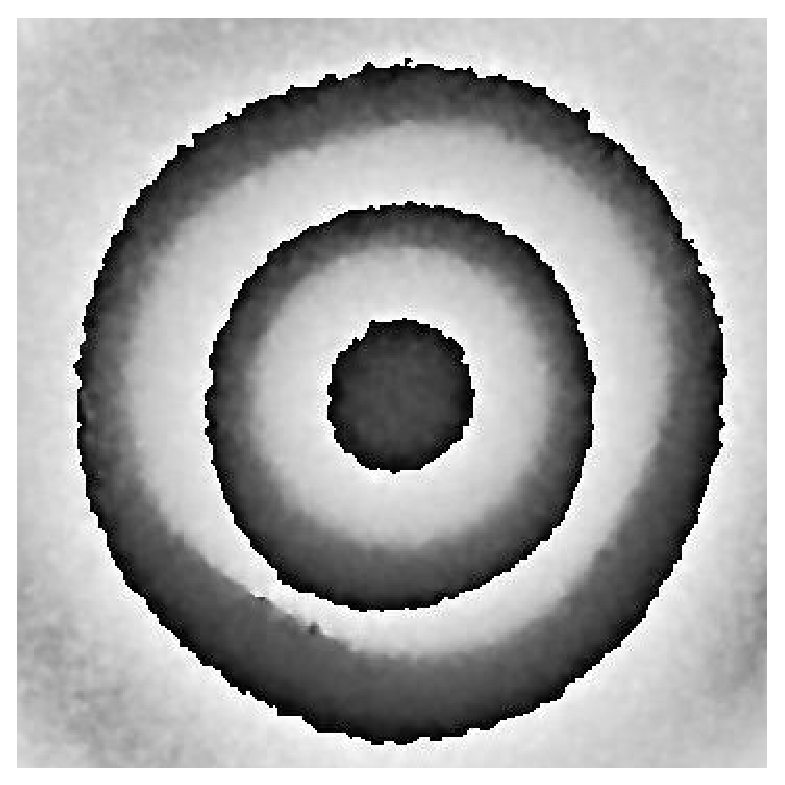
\includegraphics[scale=.43]{Chpt4_figures/fig_E1.eps}&
      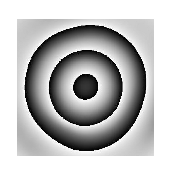
\includegraphics[scale=2.35]{Chpt4_figures/fig_E2.eps}\\
      (a) &  (b)
    \end{tabular}
  \end{center}
  \caption{Experimental wrapped phase comparison. (a) Shows the experimental
    input wrapped phase with detuning error. (b) Shows the recovered wrapped 
    phase map using the proposed PDCM.}
  \label{fig:ExperimentalPhase}
\end{figure*}

\begin{figure*}[Ht!]
  \begin{center}
      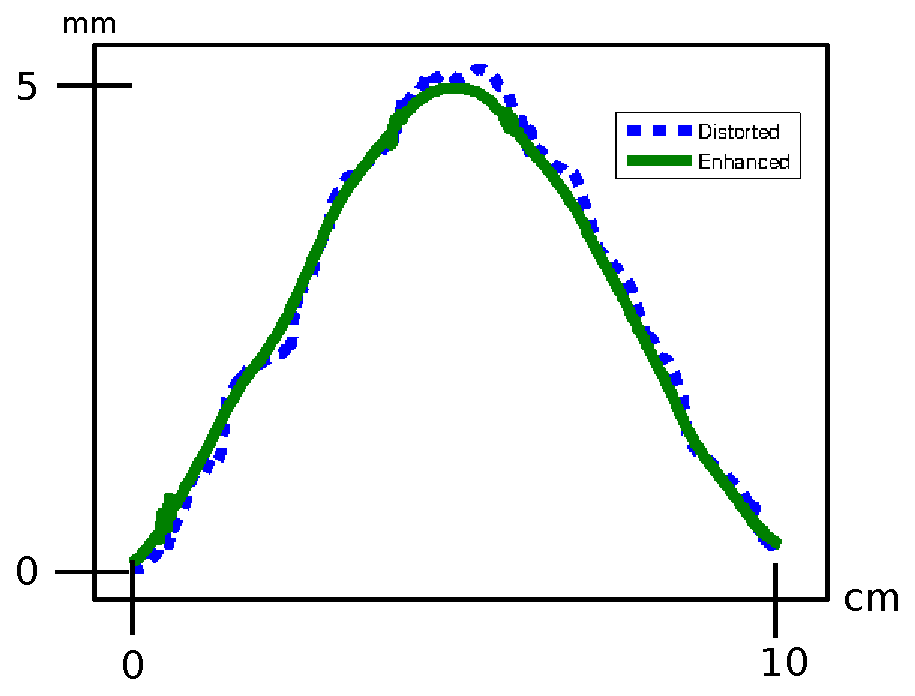
\includegraphics[scale=0.6]{Chpt4_figures/fig_E3.eps}
  \end{center}
  \caption{Comparison between an unwrapped 
    row of the distorted input and the enhanced phase; the dashed line is 
    the phase with detuning error, and the solid line is the phase processed 
    by the PDCM.}
  \label{fig:ExperimentalPhasetemp}
\end{figure*}

Finally, we show the performance in an experimental wrapped phase map. This
experimental wrapped phase map corresponds to a vibration mode of a latex
membrane excited with a horn at 1.6 kHz and with an amplitude of 1.8 V [Fig.
\ref{fig:ExperimentalPhase}(a)]. Given that the object was vibrating 
during the capture, it was not possible to correctly tune up the phase 
shift steps to $\pi/2$; as a consequence, the four step algorithm obtains 
a distorted wrapped phase map caused by the detuning. This distorted wrapped 
phase map is shown in Fig. \ref{fig:ExperimentalPhase}(a). In Fig. 
\ref{fig:ExperimentalPhase}(b), we show the performance of the proposed 
PDCM. The processing time for this phase estimation was 1.3447 seconds using
the same PC described above. As well as shown in the simulations, in Fig. 
\ref{fig:ExperimentalPhasetemp} we can see the central row of both 
unwrapped phases. As it is evident, the noise was removed and
detuning distortions have almost disappeared.

\section{Local frequency calculation in presence of noise}

\begin{figure}[Ht!] \label{fig:FaseErrorFrecuencias}
  \begin{center}
      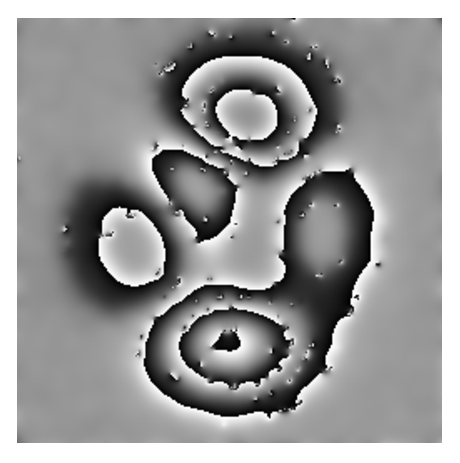
\includegraphics[scale=0.6]{Chpt4_figures/fig_mFaseErrorFrecuencias.eps}
  \end{center}
  \caption{Recovered wrapped phase using the proposed PDCM with 
  miscalculated frequencies.}
\end{figure}

In presence of noise in our input wrapped phase, the local frequencies could be
erroneously calculated given that Eqs. \ref{Eq:explicit_u} and
\ref{Eq:explicit_v} are essentially high pass filters. For example, Fig.
\ref{fig:FaseErrorFrecuencias} is the output of our proposed PDCM
when the local frequencies are miscalculated. As we can notice, the detuning
distortion and the noise were removed, but the recovered wrapped phase has
certain spurious errors product of the miscalculated local frequencies. To
avoid this problem, we propose applying a low-pass filter to our noisy input
wrapped phase. It is important to say that if we apply the low-pass filter
directly to our wrapped phase, we will lose fringe phase information. For this
reason, we propose filtering the wrapped phase as follows:
\begin{equation} \label{Eq:filtradofase}
	\hat{\phi} = \arctan \left[ \frac{\sin(\phi^\eta) * h}
	{\cos(\phi^\eta) * h} \right],
\end{equation}
where $*$ is the convolution operator, $h$ is a low-pass convolution 
kernel, $\phi^\eta$ is the noisy wrapped phase, and $\hat \phi$ is the
filtered wrapped phase, both with detuning distortions; this way of doing
the filtering allows us to keep the $2\pi$ jumps in our wrapped phase map. In
Fig. \ref{fig:filtradofase} we show the difference between these two approaches.
Fig. \ref{fig:filtradofase}(a) is the result of applying the low-pass filter 
directly to our noisy wrapped phase in Fig.
\ref{fig:SimulatedPhaseComparison}(a), while Fig. \ref{fig:filtradofase}(b)
is the outcome of filtering using Eq. \ref{Eq:filtradofase}. As it can be seen,
using the proposed approach we are able to maintain the $2\pi$ jumps, and
therefore, the fringe phase information.

\begin{figure}[Ht!]
  \begin{center}
    \begin{tabular}{c c }
      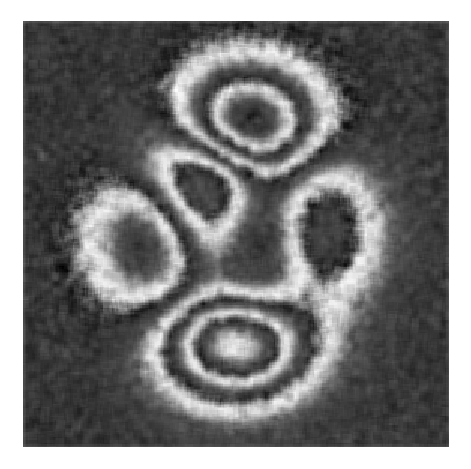
\includegraphics[scale=0.45]{Chpt4_figures/Fig_eFaseFiltradaMal.eps}&
      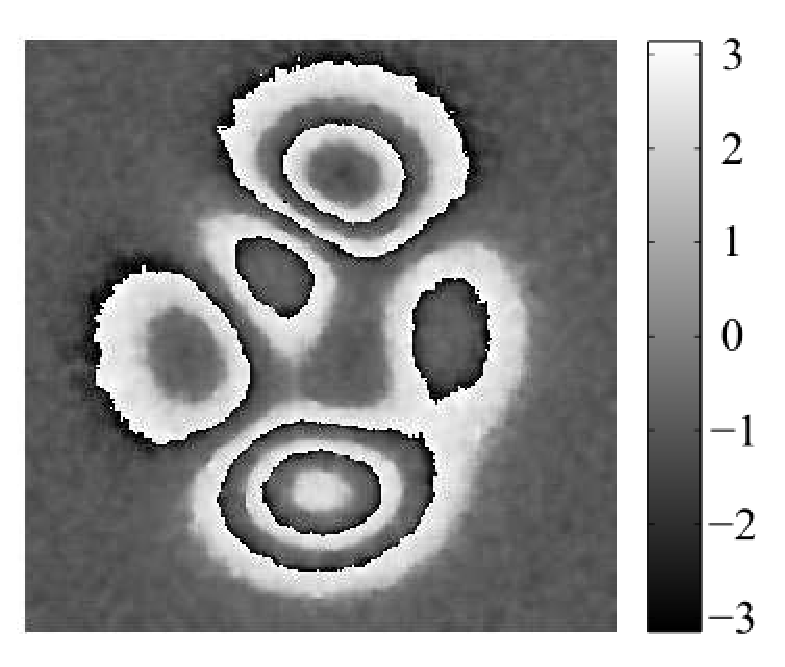
\includegraphics[scale=0.45]{Chpt4_figures/Fig_eFaseFiltrada.eps}\\
      (a) & (b)
    \end{tabular}
  \end{center}
  \caption{ Wrapped phase comparison after applying a low-pass filter to the
  noisy wrapped phase in Fig. \ref{fig:SimulatedPhaseComparison}(a). (a) 
  Shows the result of applying a gaussian filter directly to our wrapped phase,
  while in (b) we see the result of applying Eq. \ref{Eq:filtradofase}.}
  \label{fig:filtradofase}
\end{figure}

It is important to note that this process does not affect the phase information,
given that the enhanced wrapped phase is calculated using the original noisy
wrapped phase map. Also and more important, the local frequencies are a signal
with very small variations,  whereas the noise signal is the opposite.

After having removed the noise from the noisy wrapped phase, the local
frequencies can be correctly calculated. To illustrate, Fig.
\ref{fig:FaseErrorFrecuencias} shows a sequence of the calculation of three
different local frequencies during the wrapped phase refinement process.

\begin{figure}[Ht]
  \begin{center}
    \begin{tabular}{c c c}
      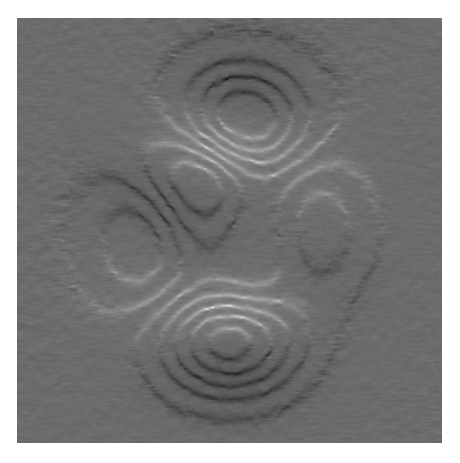
\includegraphics[scale=0.45]{Chpt4_figures/Fig_frecuencias1.eps}&
      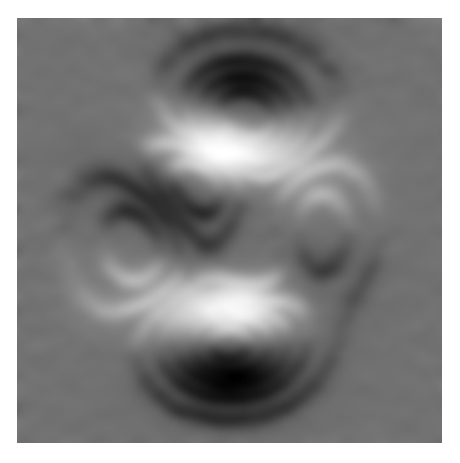
\includegraphics[scale=0.45]{Chpt4_figures/Fig_frecuencias2.eps}&
      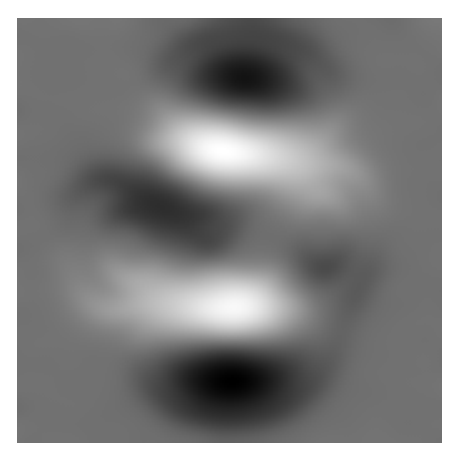
\includegraphics[scale=0.45]{Chpt4_figures/Fig_frecuencias3.eps}\\
    \end{tabular}
  \end{center}
  \caption{Example of the frequency change along the refinement process of the 
  distorted wrapped phase. For this sequence, we show the $u_(x,y)$ frequency 
  calculation using Eq. \ref{Eq:explicit_u}.}
  \label{fig:frecuencias}
\end{figure}

\section{Discussion and commentaries}
Accuracy of the wave-front estimation is the most important issue in optical 
tests. When using phase interferometry techniques, estimation accuracy depends 
on the stability of the object under test and the right calibration of the 
phase 
interferometry set-up. When the wave-front under test is moving, be it because 
of environmental perturbations or its own nature, and / or the phase 
interferometry set-up is not properly calibrated, PIDA introduce an unavoidable 
detuning error. Previous to this work, as far as we know, all PIDA have done 
their best to avoid this detuning error by means of applying different 
strategies; instead of that, here we present a method to process the distorted 
wrapped phase in order to reduce the detuning distortions introduced by the 
PIDA.

As shown in the result section, the presented PDCM considerably 
removes detuning errors using the gradient of the distorted wrapped phase as a 
priori information about the local frequencies, generating a complex signal 
with the demodulated wrapped phase, and processing it with a variant of the RQF 
to obtain a more refined demodulated wrapped phase. This process of refinement 
is carried out using the linear system of Eq. (\ref{Eq:U(f)}) iteratively. The 
proposed system looks very similar to the one used in RQF, but there 
are differences in the proposal of this work. Instead of using a global 
carrier for the entire image as in RQF, here, each pixel has its own 
frequency, in a way that the filter is locally tuned. The functional in 
RQF is non-linear, while the proposed functional [Eq. (\ref{Eq:U(f)})] 
is a linear system. Another difference is that the proposed functional is 
constructed using the demodulated wrapped phase and its local frequencies as a 
priori information. These two differences result in a stable method that 
converges in a few iterations. 

Note that using Eqs. (\ref{Eq:explicit_u}) and (\ref{Eq:explicit_v}), it is 
not necessary to unwrap the phase map to calculate the local frequencies 
$u$ and $v$. This way of calculating the local frequencies on each 
iteration speeds up the global process.

\section{Conclusions}
We have presented a method capable of reducing the 
detuning distortions of the demodulated wrapped phase from the PIDA. This 
method is an iterative process that uses the distorted wrapped phase and 
its local frequencies as a priori information. This method is stable and 
converges after a few iterations. The main contribution of the presented 
method is that it is capable of removing detuning distortions without 
eliminating wrapped phase information, which is very hard to do with 
simple low-pass filters. As it is evident in the results, the proposed 
method obtains an smooth wrapped phase map with very attenuated detuning 
distortions. The practical use of this method is that it allows one to avoid 
complex PIDA in order to obtain a wrapped phase fairly free of detuning 
distortions, or even avoid the need to recalibrate and repeat the optical 
set-up.

%Por eso es que teniendo una fase con poco ruido las eqs ... permiten ver las 
%deformaciones en la fase producidas por el detuning, esto se puede ver con
%claridad en la Fig. ...... que muestra las frecuencias en x de la fase con
%detuning. El proceso de refinamiento del PDCM lo unico que hace es hacer una
%version de la fase con variaciones mas pequeñas en la nueva fase. Teniendo asi
%una fase con la forma original y sin variaciones grandes en las frecuencias.
%En la Fig podemos ver una secuencia de tres calculos en distintos momentos del
%proceso de refinamiento de la fase. 


%\begin{thebibliography}{99}

%\bibitem{Malacara} D. Malacara, M. Servin, and Z. Malacara,
%\textit{Interferogram Analysis for Optical Testing} (Taylor \& Francis, CRC,
%2005).
 
 %\bibitem{GeneralTheory}M. Servin, J. C. Estrada, and J. A. Quiroga, “The 
 %general theory of phase shifting algorithms,” Opt. Express \textbf{17}(24), 
 %21867–21881 (2009) %doi: http://dx.doi.org/10.1364/OE.17.021867.
  
  %\bibitem{Mosino:09} J. Mosi\~{n}o, M. Servin, J. Estrada, and
  %J. Quiroga, "Phasorial analysis of detuning error in temporal phase
  %shifting algorithms," Opt. Express \textbf{17}, 5618-5623 (2009). 
  %doi: http://dx.doi.org/10.1364/OE.17.005618.
  
  %\bibitem{fringePatternAnalisys} M. Servin, J. Antonio Quiroga and M.
%Padilla, \textit{Fringe Pattern Analisys for Optical Metrology: Theory,
%Algorithms and Applications}, (Wiley-VCH, 2014).
  
  %------------
  %\bibitem{PhaseDetuning_0} J. E. Hernández and D. Malacara, "Exact linear 
  %detuning error in phase shifting algorithms," Opt. comm. \textbf{180}, 9–14 
  %(2000). 
  
  %\bibitem{PhaseDetuning_1} M. Servin, and M. Kujawinska, \textit{Modern 
  %fringe pattern analysis in Interferometry} in Handbook of Optical 
  %Engineering, D. Malacara and B. J. Thompson eds., (Marcel Dekker, 2001).
  
  %\bibitem{Mosino:10} J. Mosi\~no, D. Doblado, and D. Hern\'andez,
  %"Calculus of exact detuning phase shift error in temporal phase shifting
  %algorithms," Opt. Express  17, 15766-15771 (2009).
  
  %--------------
  %\bibitem{ShopTesting} H. Schreiber and J. H. Brunning,\textit{“Phase 
  %shifting interferometry,” in Optical Shop Testing}, D. Malacara ed., (John 
  %Wiley \& Sons, Inc., Hoboken, New Jersey 2007).
  %doi:10.1002/9780470135976.ch14.
  
  %\bibitem{AccuracyPSI_1} J. Van Wingerden, H. Frankena, and C. Smorenburg, 
  %"Linear approximation for measurement errors in phase shifting 
  %interferometry," Appl. Opt. \textbf{30}, 2718-2729 (1991) 
  %doi: http://dx.doi.org/10.1364/AO.30.002718.
  
  %\bibitem{deGroot:95} P. Groot, "Phase-shift calibration errors in 
  %interferometers with spherical Fizeau cavities," Appl. Opt. \textbf{34}, 
  %2856-2863 (1995) %doi: http://dx.doi.org/10.1364/AO.34.002856.

%\bibitem{Schmit:95} J. Schmit and K. Creath, “Extended averaging
% technique for derivation of error-compensating algorithms in phase-shifting
%interferometry,” Appl. Opt.\textbf{34}(19), 3610–3619 (1995). 
%doi: http://dx.doi.org/10.1364/AO.34.003610.

%\bibitem{Gutmann:98} B. Gutmann and H. Weber, "Phase-Shifter 
%Calibration and Error Detection in Phase-Shifting Applications: A New 
%Method," Appl. Opt. \textbf{37}, 7624-7631 (1998).
%doi: http://dx.doi.org/10.1364/AO.37.007624.

%\bibitem{Servin:10} M. Servin, J. C. Estrada, and J. A. Quiroga, “Spectral 
%analysis of phase shifting algorithms,” Opt. Express \textbf{17}(19),
%16423–16428 (2009). %doi: http://dx.doi.org/10.1364/OE.17.016423.

%\bibitem{RQF} J. Marroquin, J. Figueroa, and M. Servin, "Robust 
%quadrature filters," J. Opt.  Soc. Am. A \textbf{14}, 779-791 (1997) 
%doi: http://dx.doi.org/10.1364/JOSAA.14.000779.


%%%%%%%%%%%%%%%%%% Old references %%%%%%%%%%%%%%%%%%
  %\bibitem{AccuracyPSI_0} J. Schwider, R. Burow, K. Elssner, J. Grzanna, R. 
%Spolaczyk, and K. Merkel, "Digital wave-front measuring interferometry: 
%some systematic error sources," Appl. Opt. \textbf{22}, 3421-3432 (1983).

%\bibitem{AccuracyPSI_1} K. Kinnstaetter, A. Lohmann, J. Schwider, and N. 
%Streibl, "Accuracy of phase shifting interferometry," Appl. Opt. 
%\textbf{27}, 5082-5089 (1988).


%\bibitem{Morgan} C. Morgan, "Least-squares estimation in
%  phase-measurement interferometry," Opt.  Lett. \textbf{7}, 368-370
%  (1982).

%\bibitem{Hariharan} P. Hariharan, B. Oreb, and T. Eiju, "Digital
%  phase-shifting interferometry: a simple error-compensating phase
%  calculation algorithm," Appl. Opt. \textbf{26}, 2504-2506 (1987).

%\bibitem{Okada} K. Okada, A. Sato, and J. Tsujiuchi, "Simultaneous
%  calculation of phase distribution and scanning phase shift in phase
%  shifting interferometry," Opt.  Commun. \textbf{84}, 118-124 (1991).

%\bibitem{Kong} I.-B. Kong. "General algorithm of phase-shifting
%  interferometry by iterative least-squares fitting". Opt. Eng.,
%  \textbf{34}:183, 1995.

%\bibitem{Wang_AIA} Z. Wang and B. Han, "Advanced iterative algorithm
%  for phase extraction of randomly phase-shiftedinterferograms,"
%  Opt. Lett. \textbf{29}, 1671-1673 (2004).

%\bibitem{Mariano} R. Legarda-Saenz and M. Rivera, "Fast half-quadratic
%  regularized phase tracking for nonnormalized fringe patterns,"
%  J. Opt. Soc. Am. A \textbf{23}, 2724-2731 (2006).
  
%\bibitem{Estrada} J. Estrada, M. Servin, and J. Quiroga, "Easy and
%  straightforward construction of wideband phase-shifting algorithms
%  for interferometry," Opt. Lett.  \textbf{34}, 413-415 (2009).

%\bibitem{self_tuning} J. Estrada, M. Servin, and J. Quiroga, "A
%  self-tuning phase-shifting algorithm for interferometry,"
%  Opt. Express \textbf{18}, 2632-2638 (2010).

%\bibitem{Medina} Orlando Medina, Julio C. Estrada and Manuel Servin
%  "Regularized self-tuning phase demodulation for phase-shifting
%  interferometry with arbitrary phase shifts", Proc. SPIE
%  \textbf{8493}, Interferometry XVI: Techniques and Analysis, 84930K
%  (September 13, 2012); doi:10.1117/12.929756.
    
%\bibitem{RAPS} O. Medina, J. Estrada, and M. Servin, "Robust adaptive 
%phase-shifting demodulation for testing moving wavefronts," Opt. Express  
%\textbf{21}, 29687-29694 (2013).

  % \bibitem{Xu} J. Xu, Q. Xu, and L. Chai, "Iterative algorithm for
  %   phase extraction from interferograms with random and spatially
  %   nonuniform phase shifts," Appl. Opt.  \textbf{47}, 480-485
  %   (2008).


%\bibitem{AQF} J. Marroquin, M. Servin, and R. Rodriguez-Vera,
%  "Adaptive quadrature filters and the recovery of phase from fringe
%  pattern images," J. Opt. Soc. Am. A \textbf{14}, 1742-1753 (1997).

  % \bibitem{AQF_mult} J. Marroquin, M. Servin, and R. Rodriguez Vera,
  %   "Adaptive quadrature filters for multiple phase-stepping
  %   images," Opt. Lett.  \textbf{23}, 238-240 (1998).
 
  
%\end{thebibliography}